\documentclass[11pt,a4paper]{article}

\usepackage[T1]{fontenc}
\usepackage[utf8]{inputenc}
\usepackage[a4paper,margin=1in]{geometry}
\usepackage{graphicx}
\usepackage{float}
\usepackage[hidelinks]{hyperref}
\usepackage{parskip}
\usepackage{titlesec}

\titleformat{\section}{\large\bfseries}{\thesection.}{0.5em}{}
\titleformat{\subsection}{\normalsize\bfseries}{\thesubsection.}{0.5em}{}

\title{Architecture Report\\Activite 3 -- Layered Swing Application with MVP}
\author{HIMEUR Idris -- DIAR Adem \\ 2CS SIQ1 2025/2026}
\date{\today}

\begin{document}

\maketitle
\tableofcontents
\newpage

\section{Introduction}

This report documents the implemented architecture of \texttt{activite3}. The system is a single Java Swing desktop application, structured with explicit layers and interface-based boundaries. The source root is \texttt{activite3/src/calculator/}, and the entry point is \texttt{calculator.app.CalculatorApplication}. The build scripts compile \texttt{src/} to \texttt{out/} and run the application with local classpath dependencies \texttt{out} and \texttt{lib/interpreter.jar}.

The architectural objective is to separate concerns while preserving the calculator behavior. The presentation layer follows MVP with \texttt{CalculatorView}, \texttt{SwingCalculatorView}, and \texttt{CalculatorPresenter}. The service layer orchestrates use cases through \texttt{CalculatorService} and \texttt{CalculatorApplicationService}. External computation is isolated behind \texttt{ComputationGateway} and implemented by \texttt{InterpreterComputationGateway}. Trace persistence is isolated behind \texttt{TraceRepository} and implemented by \texttt{FileTraceRepository}, which writes a fixed-width UTF-8 table to \texttt{data/track.trc}.

\section{Development View}

The development view is organized by packages that correspond to technical responsibilities: \texttt{app}, \texttt{presentation.view}, \texttt{presentation.presenter}, \texttt{service}, \texttt{adapter}, \texttt{persistence}, and \texttt{domain}. The app layer wires concrete implementations in \texttt{CalculatorApplication.main(...)}.

MVP is explicit in presentation. \texttt{CalculatorView} defines the UI contract, and \texttt{SwingCalculatorView} provides the Swing implementation with labels and controls \texttt{Nombre 1}, \texttt{Nombre 2}, \texttt{Somme}, \texttt{Produit}, \texttt{Factoriel}, \texttt{Nombre Aleatoire}, \texttt{Trace}, and \texttt{Quitter}. \texttt{CalculatorPresenter} binds actions, validates input, delegates business operations to \texttt{CalculatorService}, and updates the view.

Interface-based boundaries reduce direct coupling: presenter depends on \texttt{CalculatorView} and \texttt{CalculatorService}; \texttt{CalculatorApplicationService} depends on \texttt{ComputationGateway} and \texttt{TraceRepository}. The adapter \texttt{InterpreterComputationGateway} implements \texttt{ComputationGateway} and is the integration point with \texttt{interpreter.Evaluator} for \texttt{add}, \texttt{multiply}, and \texttt{factorial} using postfix expressions. The \texttt{random()} method is local and uses \texttt{java.util.Random} with \texttt{nextInt(10000)}.

The domain model is intentionally compact: \texttt{OperationType} captures operation categories and display names, and \texttt{TraceEntry} captures operation operands and result values used by service and persistence.

\begin{figure}[H]
  \centering
  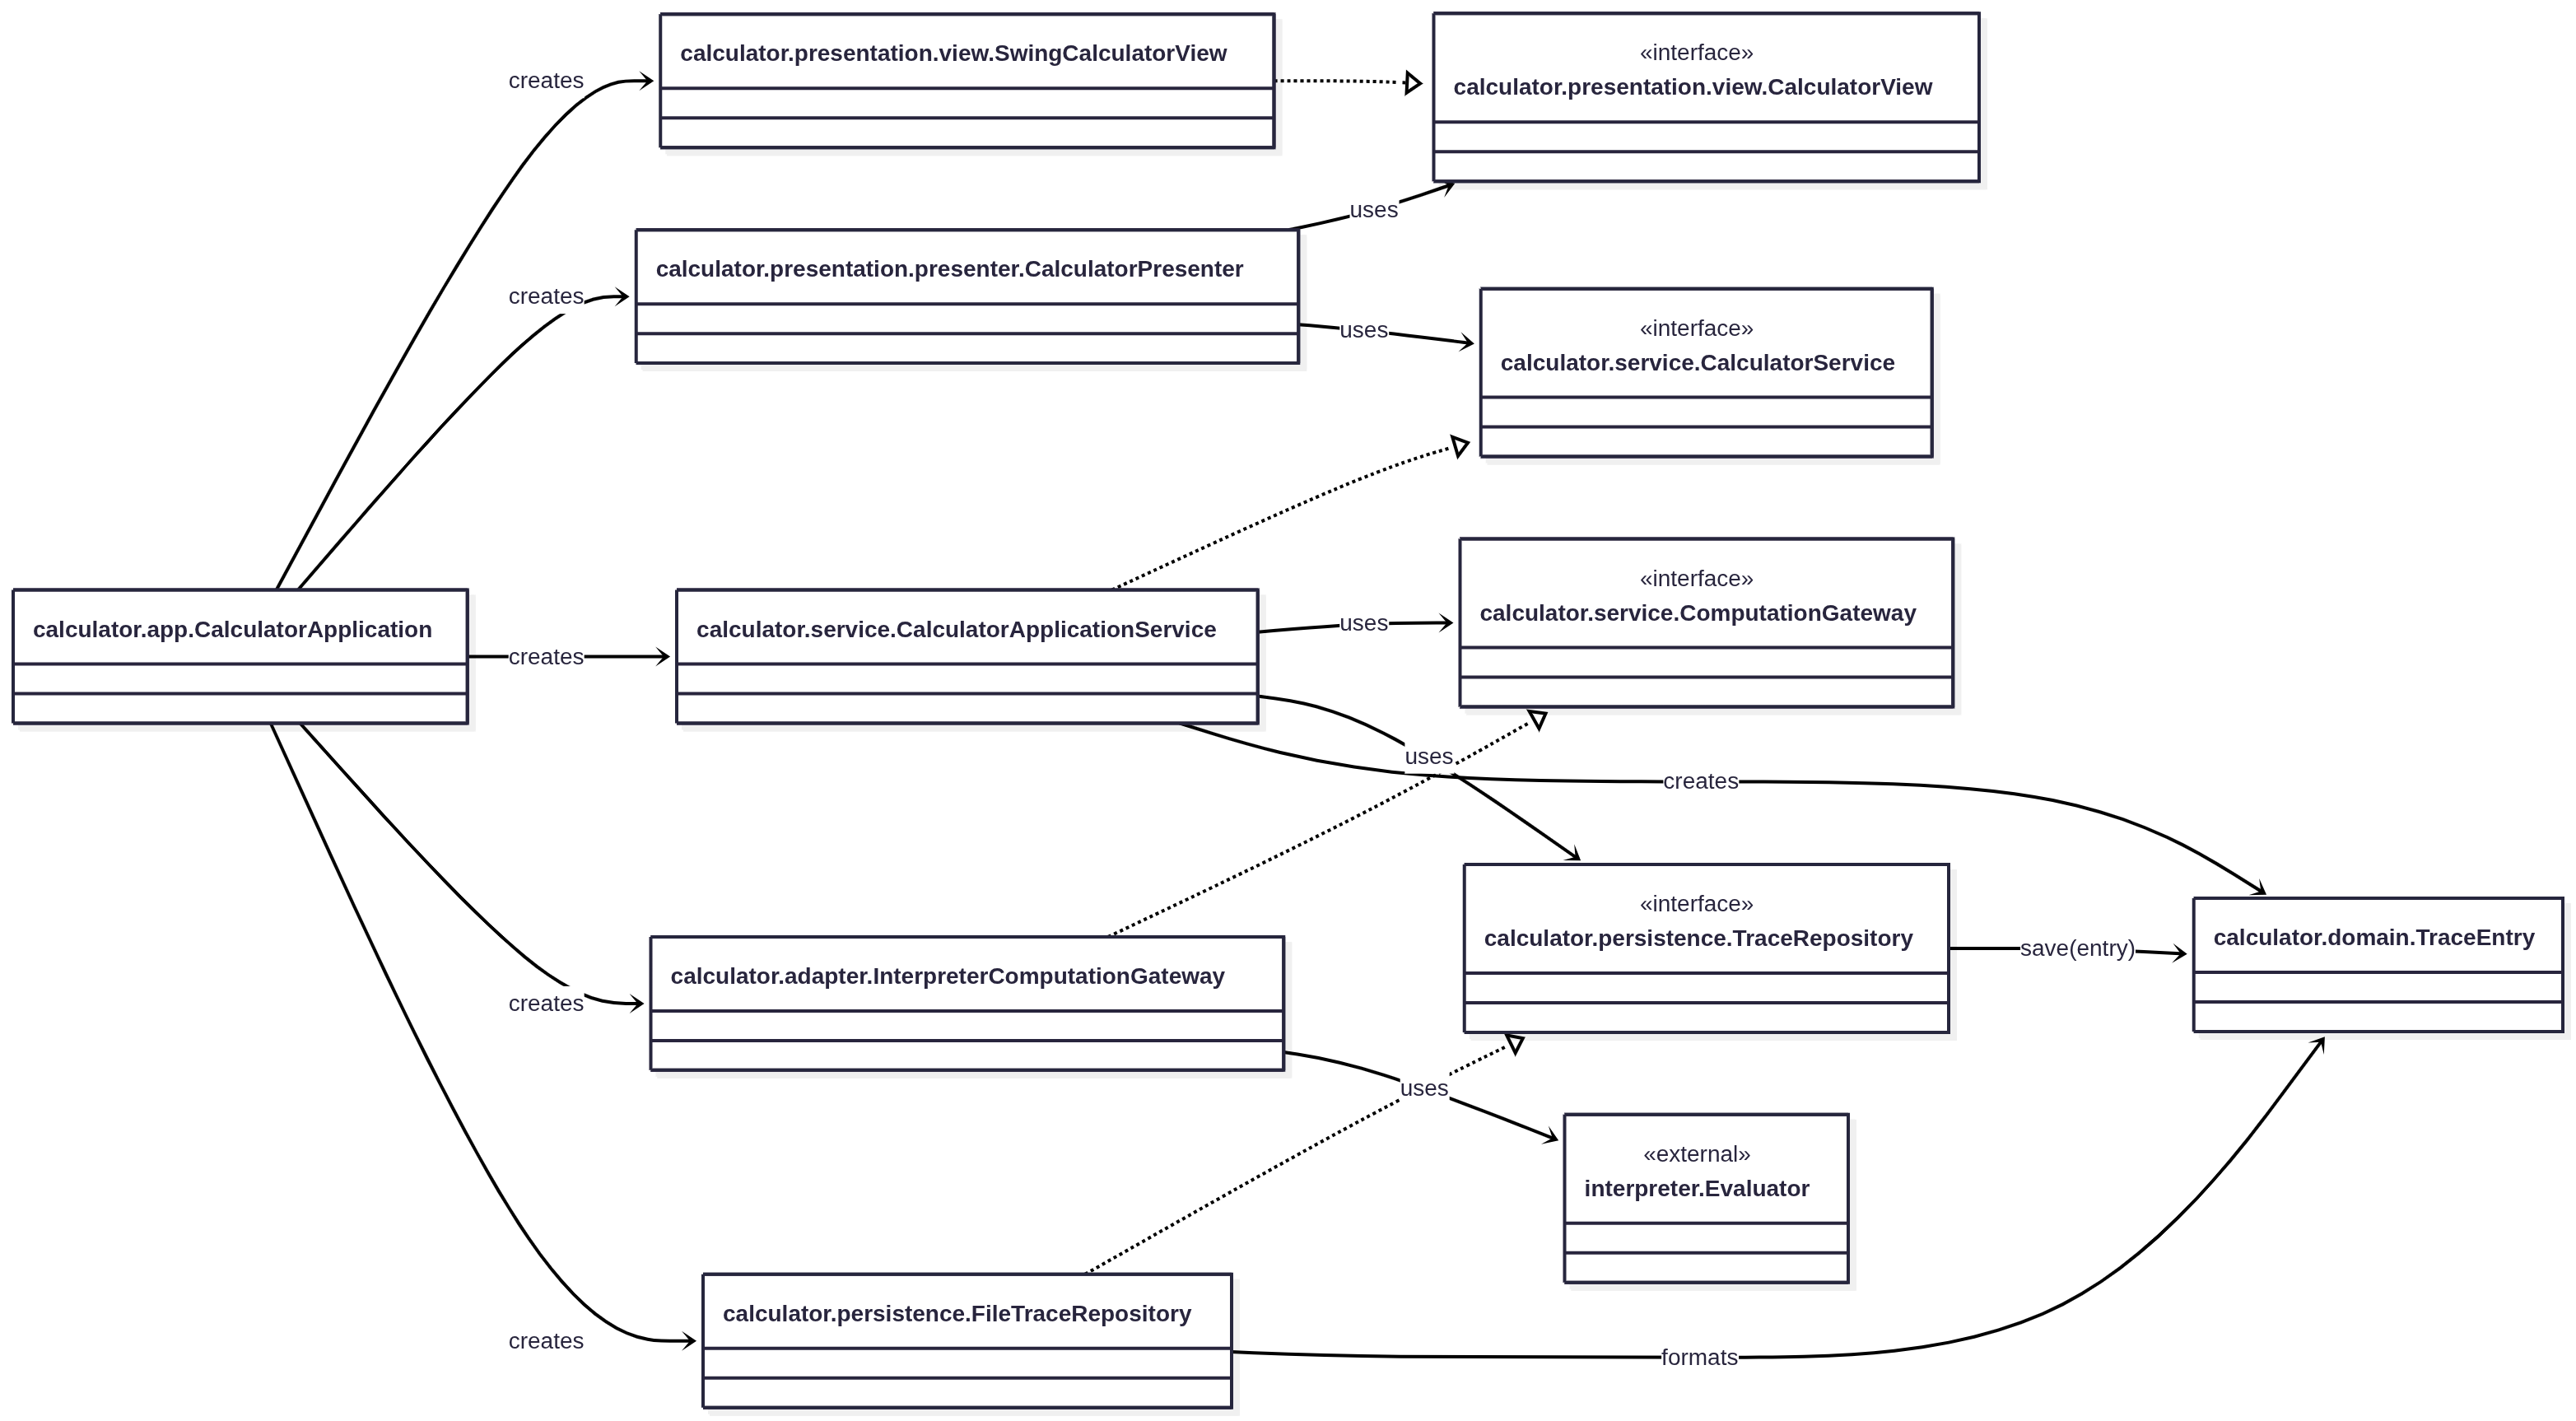
\includegraphics[width=0.98\textwidth]{diagrams/images/development_view.png}
  \caption{Development view of \texttt{activite3}: layered structure, MVP in presentation, and interface-based dependencies.}
  \label{fig:development-view}
\end{figure}

\section{Execution View}

At runtime, the application executes as one local JVM process. The UI is initialized through \texttt{SwingCalculatorView.runOnUiThread(...)} and displayed by the app layer. For operations \texttt{Somme}, \texttt{Produit}, and \texttt{Factoriel}, the flow is: user action in \texttt{SwingCalculatorView}, callback to \texttt{CalculatorPresenter}, service invocation on \texttt{CalculatorApplicationService}, delegation to \texttt{InterpreterComputationGateway}, evaluation through \texttt{interpreter.Evaluator}, persistence by \texttt{FileTraceRepository}, and UI update with \texttt{Resultat: ...}.

For \texttt{Nombre Aleatoire}, execution follows the same presentation and service path, but computation in the adapter uses \texttt{java.util.Random} directly rather than the interpreter. For \texttt{Trace}, the presenter calls \texttt{loadTraceAsText()}, which delegates to \texttt{TraceRepository.readAllAsText()} and returns the full trace text table for display.

Every computed result is persisted as a fixed-width text row. This keeps separators aligned and improves human readability in both file content and UI trace area.

\begin{figure}[H]
  \centering
  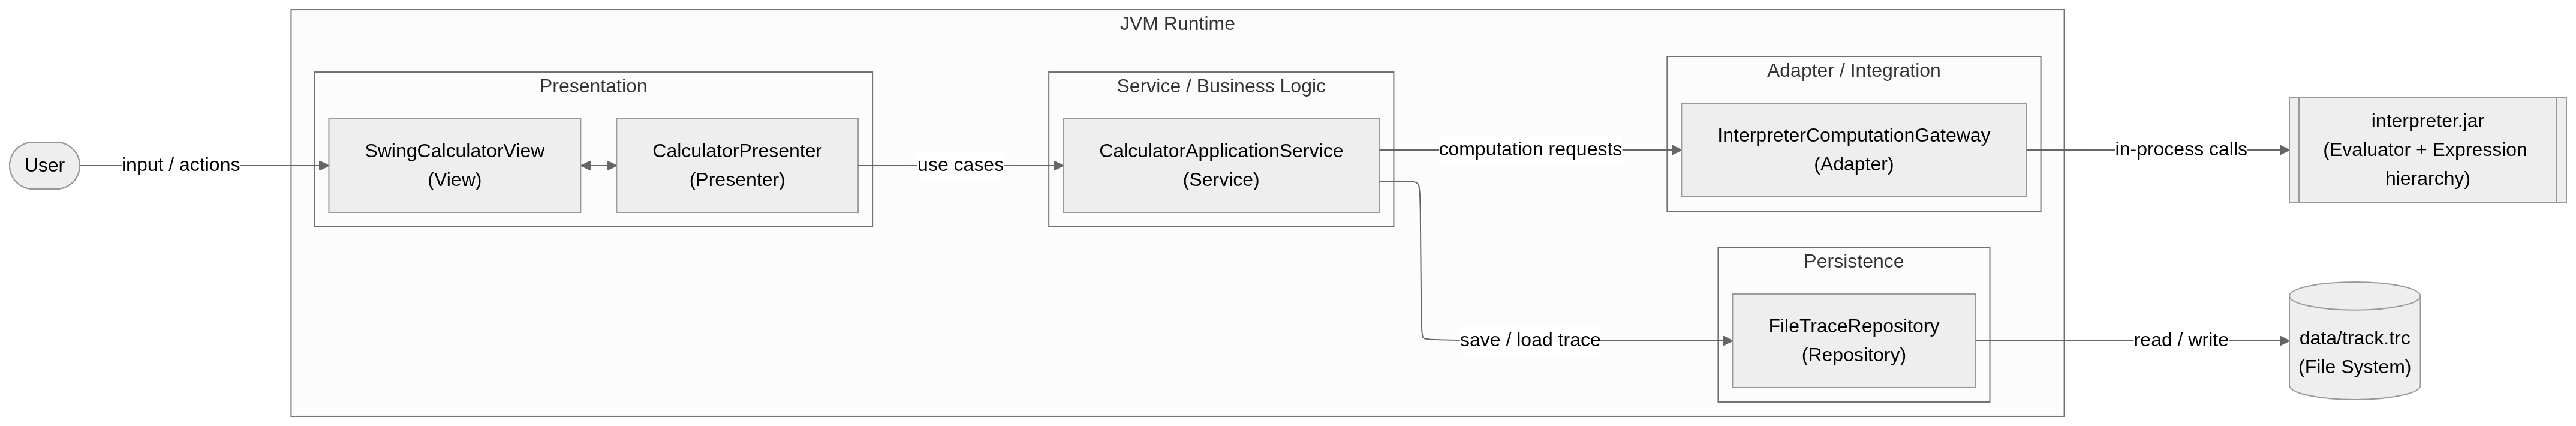
\includegraphics[width=0.98\textwidth]{diagrams/images/execution_view.png}
  \caption{Execution view: end-to-end flow from UI action to service orchestration, computation, persistence, and UI update.}
  \label{fig:execution-view}
\end{figure}

\section{Deployment View}

Deployment is intentionally minimal and local. The application runs on a single workstation with one JVM process. The external dependency \texttt{lib/interpreter.jar} is loaded as a local library. The trace is persisted in the local file \texttt{data/track.trc}.

There is no server node, no distributed runtime, no remote API call, and no database service. The architecture is therefore suitable for a standalone academic desktop application where execution, dependency loading, and persistence all occur on the same machine.

\begin{figure}[H]
  \centering
  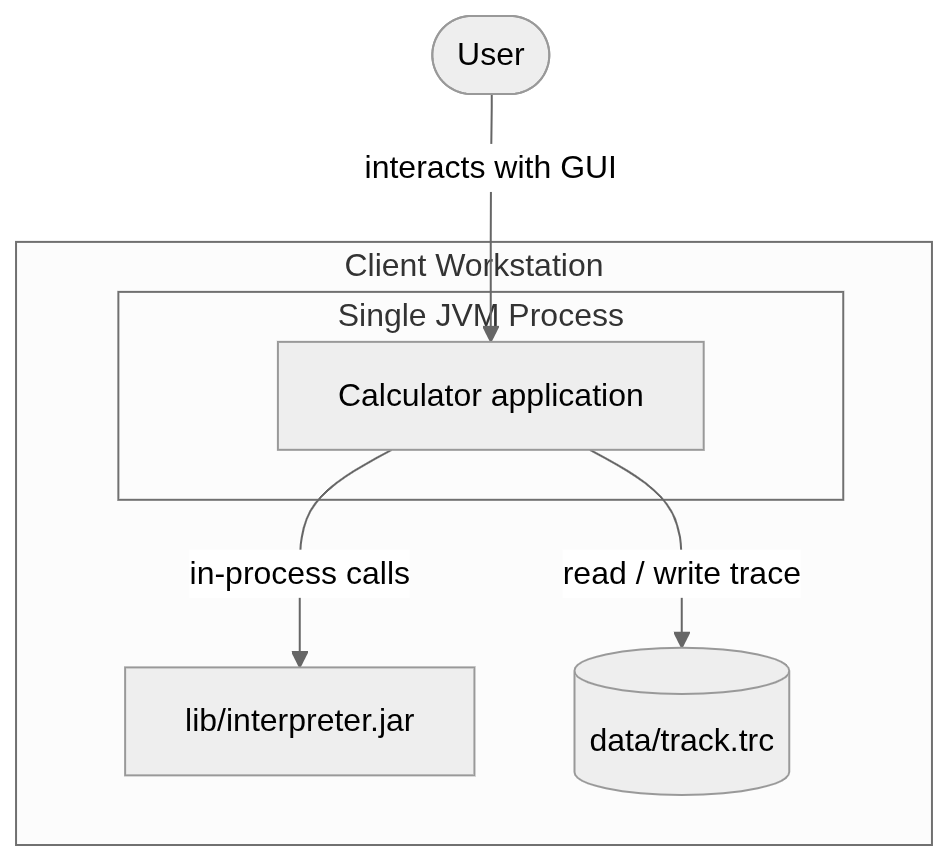
\includegraphics[width=0.95\textwidth]{diagrams/images/deployment_view.png}
  \caption{Deployment view: single-machine desktop runtime with local JAR dependency and local trace file persistence.}
  \label{fig:deployment-view}
\end{figure}

\section{Figure References in Text}

Figure~\ref{fig:development-view} summarizes static structure and interface boundaries.
Figure~\ref{fig:execution-view} shows the runtime control path for computation and trace loading.
Figure~\ref{fig:deployment-view} presents the local, single-node deployment model.

\section{Conclusion}

The implemented \texttt{activite3} architecture is a layered Swing desktop design with MVP in the presentation layer and clear interface-based integration boundaries. The service layer centralizes use-case orchestration, the adapter isolates interpreter-specific computation logic, and persistence remains independent from Swing while storing trace data in a readable fixed-width text table. This structure improves clarity, testability at boundary level, and maintainability while preserving the intended functional behavior.

\end{document}
